%  !TeX  root  =  user_guide.tex

\section{Plugin MapServer Export}\label{sec:mapserver_export}

% when the revision of a section has been finalized, 
% comment out the following line:
%\updatedisclaimer

Si può usare QGIS per comporre la propria mappa, aggiungendo e arrangiando i layer, simbolizzandoli, 
personalizzando i colori, e infine creare un map file per Mapserver per la pubblicazione sul web. 

\subsection{Creare il file Progetto}

Il Plugin MapServer Export opera su un progetto QGIS salvato e \textbf{non} sui contenuti correnti 
della vista mappa e della legenda: questo ha generato confusione in diversi utenti.
Prima di cominciare ad utilizzare il plugin, è necessario predisporre i layer vettoriali e raster 
che si intende usare in MapServer e salvare queste impostazioni in un file di progetto QGIS.

\begin{figure}[ht]
\centering
  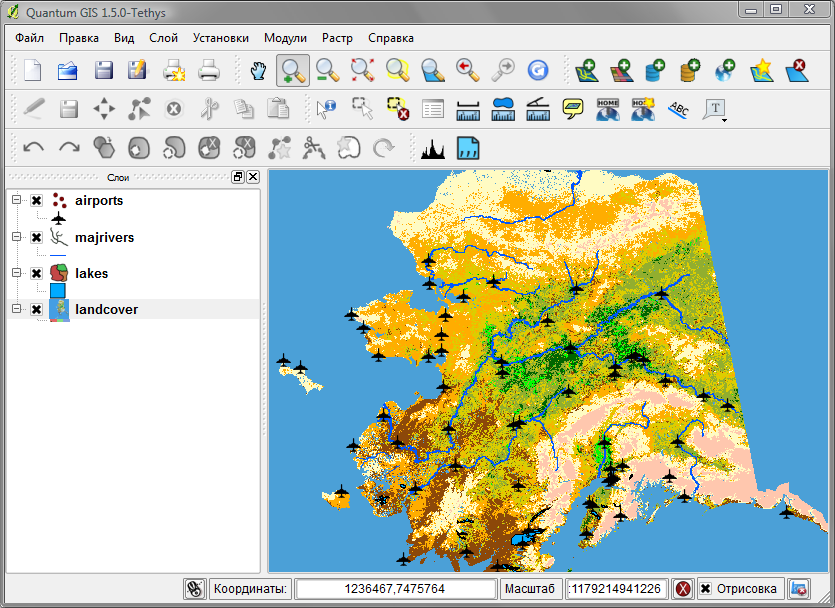
\includegraphics[clip=true, width=12cm]{mapserver_export_qgis}
   \caption{Organizzazione di layer vettoriali e raster per un file di progetto QGIS \wincaption}
  \label{fig:mapserver_export_qgs}
\end{figure}

L'esempio seguente mostra brevemente come creare un semplice progetto da usare per il mapfile di MapServer. 
Vengono usati file vettoriali e raster dal dataset campione di QGIS (\ref{label_sampledata}).

\begin{enumerate}
\item Aggiungere il layer raster \filename{landcover.tif} cliccando su 
\toolbtntwo{mActionAddRasterLayer}{Aggiungere raster}.
\item Aggiungere gli shapefile \filename{lakes.shp, majrivers.shp} e 
\filename{airports.shp} cliccando su \toolbtntwo{mActionAddNonDbLayer}{Aggiungi vettore} .
\item Cambiare lo stile dei layer (Figura~\ref{fig:mapserver_export_qgs})
\item Salvare in un nuovo progetto con nome \filename{mapserverproject.qgs} usando 
\mainmenuopt{File} > \dropmenuopttwo{mActionFileSave}{Salva progetto}.
\end{enumerate} 

\subsection{Creazione del Map File}

Lo strumento \filename{msexport} per esportare un file di progetto QGIS in un mapfile di MapServer 
è installato nella directory 'bin' di QGIS e può essere usato indipendentemente da QGIS stesso. 
In QGIS, invece, bisogna attivare il plugin utilizzando il Gestore QGIS Plugin 
(Sezione \ref{sec:load_core_plugin}).

\begin{figure}[ht]
\centering
  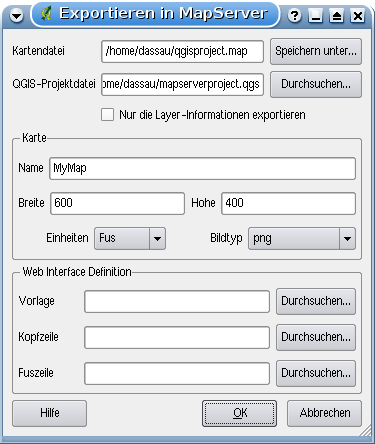
\includegraphics[clip=true, width=9cm]{mapserver_export_dialog}
  \caption{Finestra di dialogo MapServer Export \nixcaption}
  \label{fig:mapserver_export_dialog}
\end{figure}

\begin{description}
\item [Progetto QGIS] \mbox{}\\
È possibile attivare la casella di controllo \checkbox{Usa progetto corrente}, oppure selezionare un 
progetto precedentemente salvato cliccando su \button{Sfoglia...}
\item [Map file] \mbox{}\\
Scegliere un nome per il mapfile da creare. Si può usare \button{Salva con nome...} per selezionare 
la directory in cui si vuole che il file venga creato. 
\item [Nome mappa] \mbox{}\\
	Un nome per la mappa. Questo nome è usato come prefisso per tutte le immagini generate dal mapserver.
\item [Larghezza mappa] \mbox{}\\
Larghezza dell'immagine di output in pixel.
\item [Altezza della mappa] \mbox{}\\
Altezza dell'immagine di output in pixel.
\item [Unità della mappa] \mbox{}\\
Unità di misura per l'output.
\item [Tipo di immagine] \mbox{}\\
Formato dell'immagine di output generata da MapServer.
\item [Modello] \mbox{}\\
Percorso completo al template Mapserver che sarà usato con il mapfile.
\item [Titolo] \mbox{}\\
Percorso completo al file intestazione di Mapserver che sarà usato con il mapfile.
\item [Piè di pagina] \mbox{}\\
Percorso completo al file piè di pagina di Mapserver che sarà usato con il mapfile.
\end{description}

Soltanto \filename{Map file} e \filename{File di progetto QGIS} sono richiesti per creare un 
mapfile, tuttavia omettendo gli altri parametri ci si potrebbe ritrovare con un mapfile non funzionante.
Nonostante QGIS sia capace di creare un mapfile da un file di progetto, potrebbe essere necessario 
qualche successivo aggiustamento per raggiungere il risultato ottimale. 
Nell'esempio che segue, viene mostrato come creare un mapfile a partire dal progetto
\filename{mapserverproject.qgs} precedentemente salvato (Figura~\ref{fig:mapserver_export_dialog}):

\begin{enumerate}
  \item Aprire la finestra di dialogo \dialog{Esporta per MapServer} cliccando su
  \toolbtntwo{mapserver_export}{MapServer Export}.
  \item Assegnare il nome \filename{qgisproject.map} al nuovo mapfile.
  \item Selezionare il progetto QGIS \filename{mapserverproject.qgs}.
  \item Assegnare un nome alla mappa.
  \item Inserire \filename{600} per la larghezza e \filename{400} per l'altezza.
  \item Impostare le unità di misura in metri.
  \item Scegliere 'png' come tipo d'immagine.
  \item Cliccare su \button{OK} per generare il mapfile \filename{qgisproject.map}. 
\end{enumerate}

Si può visualizzare il mapfile con qualsiasi editor o visualizzatore di testo. 
Se si apre il file, si noterà che lo strumento d'esportazione aggiunge i metadati necessari 
per rendere il nostro servizio web compatibile con le specifiche WMS. 

\subsection{Testare il File Mappa}

Si può testare il risultato fin qui ottenuto usando lo strumento \filename{shp2img} per creare 
un'immagine dal mapfile. \filename{shp2img} è parte di MapServer e FWTools. 
Per creare un'immagine dalla mappa:

\begin{itemize}[label=--]
\item Aprire un terminale
\item Navigare nella cartella cui è stata salvato il mapfile
\item Lanciare \filename{shp2img -m qgisproject.map -o mapserver\_test.png} e visualizzare l'immagine 
\end{itemize}
 
Il comando crea un file PNG con tutti i layer inclusi nel progetto QGIS: l'estensione spaziale dell'immagine
sarà la stessa di quella del progetto. 
Come si vede in Figura~\ref{fig:mapserver_export_test}, tutte le informazioni eccetto i simboli 
degli aeroporti sono incluse.

\begin{figure}[ht]
\centering
  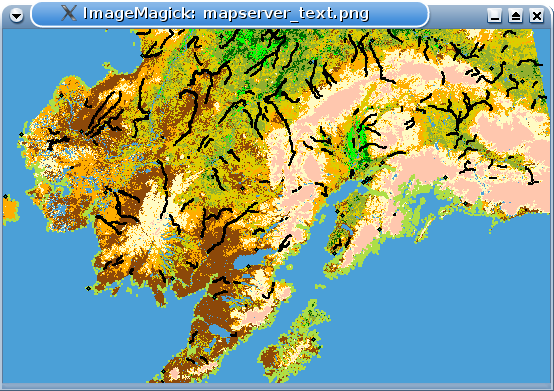
\includegraphics[clip=true, width=10cm]{mapserver_export_test}
  \caption{PNG di test creato con shp2img \nixcaption}
  \label{fig:mapserver_export_test}
\end{figure}

Se si prevede di usare il mapfile per richieste WMS standard, probabilmente non sarà necessario alcun adattamento. 
Se invece si prevede di usarlo con un modello di mappa o un'interfaccia personalizzata, potrebbe essere 
necessario del lavoro manuale. Per vedere come è facile utilizzare QGIS per offrire servizi di webmapping, 
si veda il video di Christopher Schmidt. Egli usa una vecchia versione di QGIS (0.8), 
ma le operazioni sono facilmente adattabili ad una qualsiasi versione più nuova.
\footnote{\url{http://openlayers.org/presentations/mappingyourdata/}}

\FloatBarrier